\documentclass{article}

\usepackage{enumitem}
\setlist[enumerate, 1]{label=(\alph*)}
\setlist[enumerate, 2]{label=\arabic*.}

\usepackage{tikz}
\usetikzlibrary{er, graphs}

\usepackage{minted}

\title{
    15-415/615 - Database Applications

    Answers to Homework 7
}
\author{Shangning Xu}

\begin{document}

\maketitle

\newpage

\section*{Phase 1 - Deliverables - ph1}

\begin{enumerate}
    \item Document forms:

    \begin{verbatim}
D1: user login and registration
  user name
  password

D2: user record
  user id
  user name
  password

D3: new paper
  user name
  paper title
  paper authors
  paper description
  paper text content
  upload time
  List-of:
    tag

D4: paper record
  paper id
  user id
  paper title
  paper authors
  paper description
  paper text content
  upload time
  List-of:
    user id
    like time
  List-of:
    tag

D5: paper operation
  paper id

D6: result size
  result size

D7: user time line
  paper title
  paper id
  paper authors
  paper description
  upload time
  number of likes
  List-of:
    tag

D8: paper results
  paper id
  paper title
  paper authors
  paper description
  upload time

D9: search query
  keyword
  result size

D10: search by tag
  tag
  result size

D11: tag result
  tag

D12: user paper operation
  paper id
  user id
  time

D13: user operation
  user id

D14: user statistics
  number of papers uploaded
  number of likes
  number of tags

D15: most active user
  user name

D16: tag pair
  tag1
  tag2
\end{verbatim}

    \item The ER diagram:

    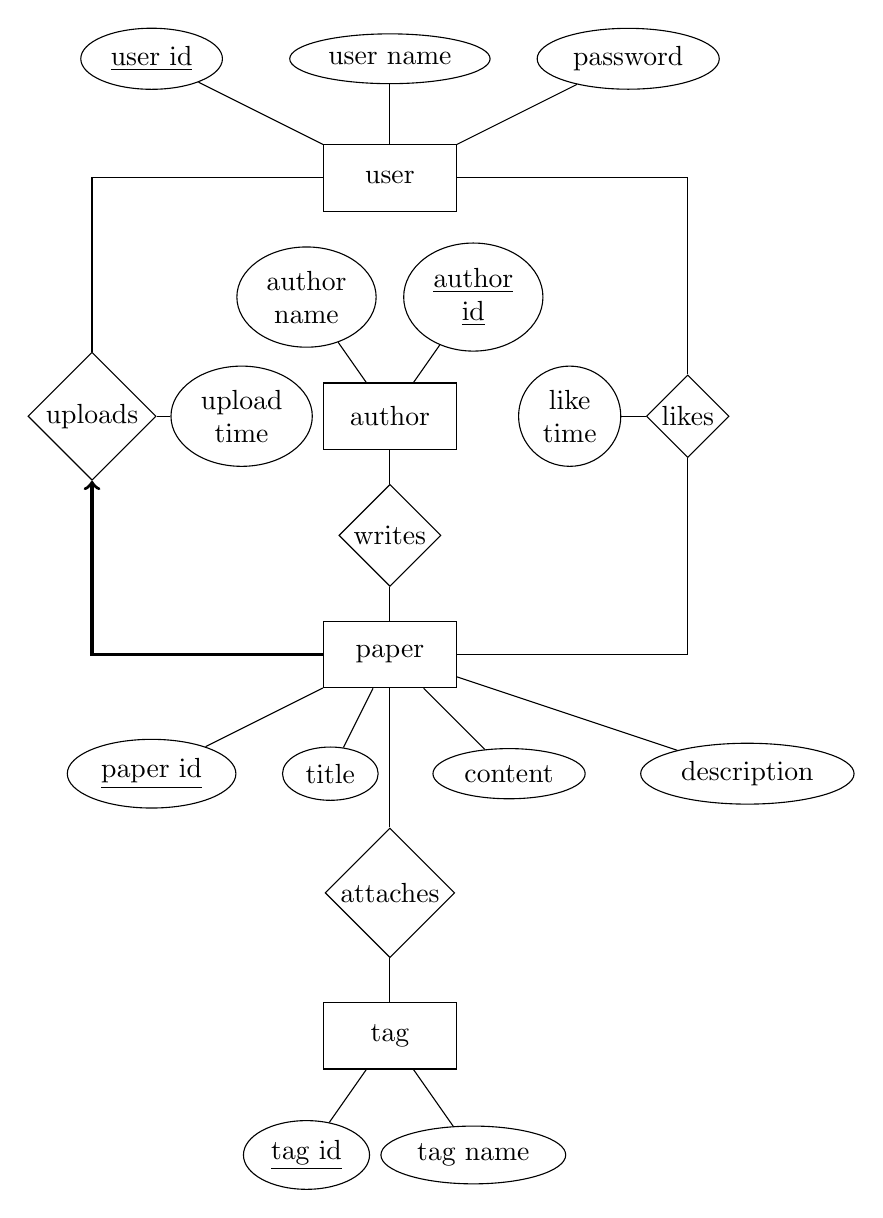
\begin{tikzpicture}
        \node [entity] (paper) {paper};
        \node [attribute] (paper id) at (-20ex, -10ex) {\underline{paper id}}
            edge (paper);
        \node [attribute] (title) at (-5ex, -10ex) {title} edge (paper);
        \node [attribute] (content) at (10ex, -10ex) {content} edge (paper);
        \node [attribute] (description) at (30ex, -10ex) {description} edge (paper);

        \node [entity] (user) at (0, 40ex) {user};
        \node [attribute] (user id) at (-20ex, 50ex) {\underline{user id}}
            edge (user);
        \node [attribute] (user name) at (0, 50ex) {user name} edge (user);
        \node [attribute] (password) at (20ex, 50ex) {password} edge (user);

        \node [relationship] (uploads) at (-25ex, 20ex) {uploads}
            [level distance=19mm] child [grow=right] {node [attribute, align=center] (upload time) {upload\\time}};
        \node [relationship] (likes) at (25ex, 20ex) {likes}
            [level distance=15mm] child [grow=left] {node [attribute, align=center] (like time) {like\\time}};
        \draw [->, very thick] (paper) -| (uploads);
        \draw (uploads) |- (user) -| (likes) |- (paper);

        \node [entity] (author) at (0, 20ex) {author};
        \node [attribute, align=center] (author name) at (-7ex, 30ex) {author\\name};
        \node [attribute, align=center] (author id) at (7ex, 30ex) {\underline{author}\\\underline{id}};
        \draw (author name) -- (author) -- (author id);
        \node [relationship] (writes) at (0, 10ex) {writes};
        \draw (author) -- (writes) -- (paper);

        \node [relationship] (attaches) at (0, -20ex) {attaches};
        \node [entity] (tag) at (0, -32ex) {tag};
        \node [attribute] (tag id) at (-7ex, -42ex) {\underline{tag id}};
        \node [attribute] (tag name) at (7ex, -42ex) {tag name};
        \draw (tag) -- (attaches) -- (paper);
        \draw (tag id) -- (tag) -- (tag name);
    \end{tikzpicture}

    \item The relation schema:
    
    \begin{quote}
        user(\underline{user id}, user name, password)

        paper(\underline{paper id}, title, content, description, uploader, upload time)

        author(\underline{author id}, author name)

        tag(\underline{tag id}, tag name)

        writes(\underline{author id, paper id})

        attaches(\underline{paper id, tag id})

        likes(\underline{user id, paper id}, like time)
    \end{quote}

    \item \begin{minted}[breaklines]{sql}
CREATE TABLE users (
    id INTEGER PRIMARY KEY,
    user_name VARCHAR(50) NOT NULL,
    password VARCHAR(32) NOT NULL
);

CREATE TABLE papers (
    id INTEGER PRIMARY KEY,
    title VARCHAR(50) NOT NULL,
    content TEXT NOT NULL,
    description VARCHAR(500),
    uploader INTEGER NOT NULL REFERENCES users(user_id),
    upload_time TIMESTAMP NOT NULL DEFAULT CURRENT_TIMESTAMP
);

CREATE TABLE authors (
    id INTEGER PRIMARY KEY,
    name VARCHAR(128) NOT NULL
);

CREATE TABLE tags (
    id INTEGER PRIMARY KEY,
    name VARCHAR(50) NOT NULL UNIQUE
);

CREATE TABLE writes (
    author_id INTEGER NOT NULL REFERENCES authors(id),
    paper_id INTEGER NOT NULL REFERENCES papers(id) ON DELETE CASCADE,
    PRIMARY KEY (author_id, paper_id)
);

CREATE TABLE attaches (
    paper_id INTEGER NOT NULL REFERENCES papers(id) ON DELETE CASCADE,
    tag_id INTEGER NOT NULL REFERENCES tags(id) ON DELETE CASCADE,
    PRIMARY KEY (paper_id, tag_id)
);

CREATE TABLE likes (
    user_id INTEGER NOT NULL REFERENCES users(id) ON DELETE CASCADE,
    paper_id INTEGER NOT NULL REFERENCES papers(id) ON DELETE CASCADE,
    like_time TIMESTAMP NOT NULL DEFAULT CURRENT_TIMESTAMP,
    PRIMARY KEY (user_id, paper_id)
);
\end{minted}

    \item \begin{enumerate}
        \item \mint[breaklines]{sql}{TRUNCATE users, papers, authors, tags, writes, attaches, likes;}
        
        \item \begin{minted}[breaklines]{sql}
INSERT INTO users (user_name, password) VALUES (<username>, <password>)
    ON CONFLICT (user_name) DO NOTHING;
\end{minted}

        \item \mint[breaklines]{sql}{SELECT FROM users WHERE user_name = <username> AND password = <password>;}
        
        \item \begin{minted}[breaklines]{sql}
WITH new_paper_id AS (
            INSERT INTO papers (title, content, description, uploader)
                VALUES (<title>, <content>, <description>, <uploader>) RETURNING id
        ),
        new_author_ids AS (
            INSERT INTO authors (name) VALUES (<author-name>) ... RETURNING id
        ),
        temp AS (
            INSERT INTO writes (author_id, paper_id)
                SELECT new_author_ids.id, new_paper_id.id FROM new_author_ids, new_paper_id
        ),
        tags_to_insert AS (VALUES (<tag name>), ...),
        inserted_tag_ids AS (
            INSERT INTO tags (name) SELECT * FROM tags_to_insert RETURNING id ON CONFLICT DO NOTHING
        ),
        all_tag_ids AS (
            SELECT id FROM tags JOIN tags_to_insert USING (name) UNION ALL SELECT * FROM inserted_tag_ids
        ),
    INSERT INTO attaches (paper_id, tag_id)
            SELECT new_paper_id.id, new_tag_ids.id FROM new_paper_id, new_tag_ids;
\end{minted}
        \item \mint[breaklines]{sql}{DELETE FROM papers WHERE id = <paper-id>;}

        \item \begin{minted}[breaklines]{sql}
SELECT id, title, description, upload_time, (SELECT COUNT(*) FROM likes WHERE paper_id = papers.id)
    FROM papers ORDER BY upload_time DESC, id LIMIT <K>;

SELECT name FROM authors JOIN writes ON id = author_id WHERE paper_id = <paper-id>;

SELECT name FROM tags JOIN attaches ON id = tag_id WHERE paper_id = <paper-id>;
\end{minted}

        \item \begin{minted}[breaklines]{sql}
SELECT id, title, description, upload_time FROM papers ORDER BY upload_time DESC, id LIMIT <K>;

SELECT name FROM authors JOIN writes ON id = author_id WHERE paper_id = <paper-id>;
\end{minted}

        \item \begin{minted}[breaklines]{sql}
SELECT id, title, description, upload_time FROM papers
    WHERE title LIKE '%<keyword>%'
        OR content LIKE '%<keyword>%'
        OR description LIKE '%<keyword>%'
    ORDER BY upload_time DESC, id LIMIT <K>;

SELECT name FROM authors JOIN writes ON id = author_id WHERE paper_id = <paper-id>;
\end{minted}

        \item \begin{minted}[breaklines]{sql}
SELECT id, title, description, upload_time
    FROM tags JOIN attaches ON tags.id = tag_id JOIN papers ON paper_id = papers.id
    WHERE tags.name LIKE '%<tag name>%'
    ORDER BY upload_time DESC, id LIMIT <K>;

SELECT name FROM authors JOIN writes ON id = author_id WHERE paper_id = <paper-id>;
\end{minted}

        \item \begin{minted}[breaklines]{sql}
SELECT name FROM tags JOIN attaches ON tags.id = tag_id
    WHERE paper_id = <paper-id> ORDER BY name;
\end{minted}

        \item \begin{minted}[breaklines]{sql}
-- Like a paper.
INSERT INTO likes (user_id, paper_id) VALUES (<user-id>, <paper-id>);
-- Unlike a paper.
DELETE FROM likes WHERE user_id = <user-id> AND paper_id = <paper-id>;
\end{minted}

        \item \mint[breaklines]{sql}{SELECT COUNT(*) FROM likes WHERE paper_id = <paper-id>;}
        
        \item \begin{minted}[breaklines]{sql}
SELECT id FROM papers JOIN likes ON paper_id = id WHERE user_id = <user-id>
    ORDER BY upload_time DESC, id LIMIT <K>;
\end{minted}

        \item \begin{minted}[breaklines]{sql}
SELECT paper_id, COUNT(*) AS like_count FROM likes
    WHERE paper_id IN (SELECT id FROM papers WHERE upload_time >= <T>)
    GROUP BY paper_id ORDER BY like_count DESC, id LIMIT <K>;

SELECT name FROM authors JOIN writes ON id = author_id WHERE paper_id = <paper-id>;
\end{minted}

        \item \begin{minted}[breaklines]{sql}
WITH liked_papers AS (SELECT DISTINCT paper_id FROM likes WHERE user_id = <user-id>)
    SELECT paper_id, COUNT(*) AS like_count FROM likes
        WHERE user_id IN (SELECT DISTINCT user_id FROM likes WHERE paper_id IN liked_papers)
            AND paper_id NOT IN liked_papers
        GROUP BY paper_id ORDER BY like_count DESC, id;
\end{minted}

        \item \begin{minted}[breaklines]{sql}
WITH uploaded_papers AS (SELECT id FROM papers WHERE uploader = <user-id>)
    SELECT
        (SELECT COUNT(*) FROM uploaded_papers),
        (SELECT COUNT(*) FROM likes WHERE user_id = <user-id>),
        (SELECT COUNT(DISTINCT tag_id) FROM likes WHERE paper_id IN uploaded_papers);
\end{minted}
  
        \item \begin{minted}[breaklines]{sql}
-- (a)
SELECT user_name, upload_count FROM users JOIN (SELECT uploader, COUNT(*) as upload_count FROM papers GROUP BY uploader) ON id = uploader
    ORDER BY upload_count DESC, id LIMIT <K>;
-- (b)
SELECT name, count
    FROM tags JOIN (SELECT tag_id, COUNT(*) as count FROM attaches GROUP BY tag_id) ON id = tag_id
    ORDER BY count DESC, id LIMIT <K>;
-- (c)
WITH attaches_with_names AS (
            SELECT tag_id, name FROM tags JOIN attaches ON tags.id = tag_id
        ),
    SELECT a1.name AS tag1, a2.name AS tag2, COUNT(tag1, tag2) AS pair_count
        FROM attaches_with_names AS a1, attaches_with_names AS a2
        WHERE a1.paper_id = a2.paper_id AND a1.name < a2.name
        GROUP BY tag1, tag2 ORDER BY pair_count DESC, tag1, tag2 LIMIT <K>;
\end{minted}
    \end{enumerate}
\end{enumerate}

\newpage

\section*{Phase 2 - Deliverables - ph2}

\begin{enumerate}[start=3]
    \item Test plan:
    
    \begin{enumerate}
        \item Reset database
        
        \item Create user account (Register)
        \begin{itemize}
            \item Duplicate user names.
            \item User name too long.
            \item Password too long.
        \end{itemize}

        \item Login
        \begin{itemize}
            \item User name not found.
            \item Password incorrect.
        \end{itemize}

        \item Upload a paper with tags
        \begin{itemize}
            \item No author.
            \item No tag.
        \end{itemize}

        \item Delete a paper
        \begin{itemize}
          \item Paper not found.
          \item Associated information not deleted.
        \end{itemize}

        \item User timeline
        \begin{itemize}
            \item Correctness.
        \end{itemize}

        \item Global timeline
        \begin{itemize}
            \item Correctness.
        \end{itemize}

        \item Search for papers.
        \begin{itemize}
            \item Complete title match.
            \item Complete description match.
            \item Complete content match.
        \end{itemize}

        \item Search by a tag
        \begin{itemize}
            \item Correctness.
        \end{itemize}

        \item Get tags of a paper
        \begin{itemize}
            \item Non-existent paper.
        \end{itemize}

        \item Like/Unlike a paper
        \begin{itemize}
            \item Like liked paper.
            \item Unlike unliked paper.
            \item Non-existent paper.
        \end{itemize}

        \item Count likes
        \begin{itemize}
            \item Non-existent paper.
        \end{itemize}

        \item List favorite papers of a user
        \begin{itemize}
            \item Non-existent user.
            \item No favorite papers.
        \end{itemize}

        \item List most popular papers
        \begin{itemize}
            \item No papers in the table.
        \end{itemize}

        \item Recommend papers based on likes
        \begin{itemize}
            \item Non-existent user.
            \item Never liked any paper.
            \item Liked paper not liked by anyone else.
        \end{itemize}

        \item User statistics
        \begin{itemize}
            \item Non-existent user.
        \end{itemize}

        \item Global statistics
        \begin{itemize}
            \item No users.
            \item No tags.
            \item No papers.
        \end{itemize}
    \end{enumerate}
\end{enumerate}

\end{document}
